Knowledge of projective geometry is vital to understanding elliptic curves, as they are curves that are defined in the projective plane.
However, the definition is not too complicated.
\begin{definition}
	An elliptic curve is a regular, projective cubic curve.
\end{definition}
Here, a cubic simply means that the polynomial that defines the curve is of degree three.
So for example, $F(X,Y,Z) = X^3 + 2XYZ + 5YZ^2 + \frac{1}{2}Z^3$ defines an elliptic curve $F(X,Y,Z) = 0$. % Check this!!
\subsubsection{The Addition Law on Elliptic Curves}
Our interest in elliptic curves is mainly concentrated on a special property, unique to them.
It is possible to turn the set of points of an elliptic curve $E$ into a group by introducing a special addition law that satisfies all of the group axioms.
We do not prove this in this document for the sake of brevity but there are many proper treatments elsewhere, such as \cite{silverman2009}.
\begin{figure}[htpb]
	\centering
	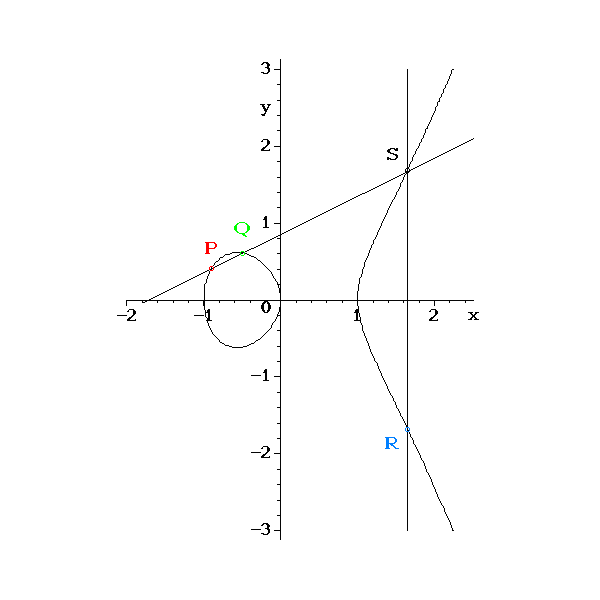
\includegraphics[scale=0.5]{addition.png}
	\caption{The chord-tangent composition law on an elliptic curve}
	\label{chord-tangent}
\end{figure}
The addition rests upon the so-called `chord-tangent~law', which is roughly illustrated in \Cref{chord-tangent}.
Since an elliptic curve is cubic and regular, by definition, every line intersects it with multiplicity exactly three.
This means that given two points (not necessarily distinct), the line on which those points lie (or the tangent line to the curve at the point, if the points are the same) will intersect the curve in exactly one other place (including the same point again, if it is a flex).
The idea of the chord-tangent law is that we can take any two points $P$ and $Q$ and define $P * Q$ to be this third point of intersection.
Does this make $E$ into a group though?

It turns out the answer is no, since associativity is not satisfied. This can be remedied, though, by defining the elliptic curve addition law as follows.

%%%%%%%%%%%%%%%%%%%%
\begin{definition}
	An elliptic curve is a non-singular cubic projective curve. For our purposes, they can all be written as $y^2 = f(x)$, where $f(x)$ is a cubic polynomial in $x$ with no repeated roots.
\end{definition}
